\documentclass{article}
\usepackage{chngpage}
\usepackage[utf8]{inputenc}
\usepackage[margin=2cm]{geometry}
\usepackage{tikz}

\title{Assignment 2: Concurrent word detector}
\author{Julien GAUTIER, Florent BORDIGNON}

\begin{document}
\maketitle
Dans ce rapport, le mot "distance" se référera à la distance
d'alignement optimal de chaine de charactère (Optimal string aligment
distance).

\section{Dictionnaire synchrone}
\subsection{Fonctionnement}
Dictionary est implémenté avec un TRIE.
Une requête search commence par verifier si mot exact existe dans le dictionnaire. Si ce n'est pas le cas, on utilise l'algorithme de Wagner-Fisher modifié de manière à prendre en compte les swaps.
Le mot recherché est écrit sur la ligne du haut du tableau.
Pour faire une recherche, on fait un parcourt profondeur du Trie. A chaque
noeud, une ligne est ajoutée. Cette algoritme permet de consever le début du
tableau en utilisant le backtracking.\\

\newenvironment{tab}{
  \begin{minipage}{0.1\paperwidth}
    \begin{tabular}{|l|r|r|r|r|}
}{
    \end{tabular}
  \end{minipage}
}
\newenvironment{tree}{
  \begin{minipage}{0.16\paperwidth}
    \begin{tikzpicture}
}{
    \end{tikzpicture}
  \end{minipage}
}
\newcommand\step[1]{
  \framebox[0.4\paperwidth]{#1}
}
\newenvironment{twosteps}{
  % Adjusting the width (by 0cm here) is neede when the margins are too
  % big...
  \begin{adjustwidth}{0cm}{0cm}
}{
  \end{adjustwidth}
}
\newcommand\nop{}

\begin{twosteps}
  \step{
    \begin{tree}
      \node {-}
      child {node [fill=red!30,label=left:$\to$] {N}
        child {node {L}}
      }
      child {node {S}
        child {node {L}
          child {node {N}}
        }
        child {node {U}}
      };
    \end{tree}
    \begin{tab}
      \hline
      \nop{}	& L	& N\\
      \hline
      N		& 1	& 1\\
      \hline
    \end{tab}
  }% \step
  \step {
    \begin{tree}
      \node {-}
      child {node [fill=red!30] {N}
        child {node [label=left:$\to$] {L}}
      }
      child {node {S}
        child {node {L}
          child {node {N}}
        }
        child {node {U}}
      };
    \end{tree}
    \begin{tab}
      \hline
      \nop{}	& L	& N\\
      \hline
      N		& 1	& 1\\
      \hline
      L		& 1	& 1\\
      \hline
    \end{tab}
  }% \step
\end{twosteps}

\begin{twosteps}
  \step{
    \begin{tree}
      \node {-}
      child {node {N}
        child {node {L}}
      }
      child {node [fill=red!30,label=left:$\to$] {S}
        child {node {L}
          child {node {N}}
        }
        child {node {U}}
      };
    \end{tree}
    \begin{tab}
      \hline
      \nop{}	& L	& N\\
      \hline
      S		& 1	& 2\\
      \hline
    \end{tab}
  }% \step
  \step {
    \begin{tree}
      \node {-}
      child {node {N}
        child {node {L}}
      }
      child {node [fill=red!30] {S}
        child {node [label=left:$\to$] {L}
          child {node {N}}
        }
        child {node {U}}
      };
    \end{tree}
    \begin{tab}
      \hline
      \nop{}	& L	& N\\
      \hline
      S		& 1	& 2\\
      \hline
      L		& 1	& 2\\
      \hline
    \end{tab}
  }% \step
\end{twosteps}

\begin{twosteps}
  \step {
    \begin{tree}
      \node {-}
      child {node {N}
        child {node {L}}
      }
      child {node [fill=red!30] {S}
        child {node {L}
          child {node [label=left:$\to$] {N}}
        }
        child {node {U}}
      };
    \end{tree}
    \begin{tab}
      \hline
      \nop{}	& L	& N\\
      \hline
      S		& 1	& 2\\
      \hline
      L		& 1	& 2\\
      \hline
      N		& 2	& 1\\
      \hline
    \end{tab}
  }% \step
  \step {
    \begin{tree}
      \node {-}
      child {node {N}
        child {node {L}}
      }
      child {node [fill=red!30] {S}
        child {node {L}
          child {node {N}}
        }
        child {node [label=left:$\to$] {U}}
      };
    \end{tree}
    \begin{tab}
      \hline
      \nop{}	& L	& N\\
      \hline
      S		& 1	& 2\\
      \hline
      U		& 2	& 2\\
      \hline
    \end{tab}
  }% \step
\end{twosteps}
\begin{flushright}
  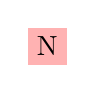
\begin{tikzpicture}
    \node [fill=red!30] {N};
  \end{tikzpicture}
  : \textit{lock} verrouillé\\
  \begin{tikzpicture}
    \node [label=left:$\to$] {N};
  \end{tikzpicture}
  : étape courante
\end{flushright}
\begin{center}
  \textit{Recherche du mot ``ln" dans le dictionnaire \{``nl", ``sln",
    ``su"\}}.
\end{center}


\subsection{Pruning}
On note:
\begin{itemize}
\item $t_a$ la taille du mot actuel
\item $t_r$ la taille du mot recherché
\item $d_a$ la distance du mot actuel au mot recherché
\item $d_m$ la meilleure distance trouvée jusqu'à présent entre un mot du dictionnaire et le mot recherché
\end{itemize}
On cherche a arréter la recherche le plus tôt possible de trois manières:
\begin{itemize}
\item Si $d_m = 1$, cela ne sert à rien de continuer car pour avoir une meilleure distance, il faudrait trouver le mot recherché dans le dictionnaire. Or la recherche par distance de Levenshtein est lancé uniquement si le mot n'existe pas tel quel dans le dictionnaire.

\textit{Exemple: Etape 2.}

\item La distance minimum entre deux mots est la différence de taille
  entre ces deux mots.
Si la taille du mot correspondant au noeud actuel du Trie est supérieure
à la taille du mot recherché plus la meilleure distance trouvée jusqu'à
présent ($t_a > t_r + d_m$), alors on peut arréter la recherche de cette branche.

\textit{Exemple: Etape 5.}

\item La distance entre le mot actuel et le mot recherché (la case en
  bas à droite du tableau) ne peut diminuer que de 1 lorsque l'on ajoute
  une ligne.
Donc il faut ajouter au minimum $d_a - d_m$ caractères pour avoir un nouveau minimum.
Ce nouveau minimum potentiel aura un taille égal à $t_a + (d_a - d_m)$.
Si cette taille est supérieure à $t_r + d_m$,
alors il n'y a aucune chance pour que cette branche puisse trouver un
nouveau minimum.
On peut donc s'arréter.

\textit{Exemple: Etape 4.}
\end{itemize}

\subsection{Fine-grained locking}
26 branches partent de la racine du Trie.
Une opération peut travailler soit sur la racine, soit sur le reste de
l'arbre.
Si l'opération travaille sur la racine, un lock global assure lui assure
l'exclusivité du dictionnaire.
Si l'opération ne travail pas sur la racine (le cas le plus fréquent),
il travaille donc sur l'un des 26 fils de la racine.
Chacun de ces fils peut être lock individuellement.
Si l'opération est une recherche le compteur des readers pour cette
branche est augmenté de 1.
Si l'opération modifie l'arbre, alors il attend qu'il n'y ai plus aucun
lecteur sur cette branche, puis il lock la branche.

\section{AsyncDictionary}
Pour assurer la sequentialité du dictionaire, nous avons utilisé un
système de ticket.
Il y a un compteur pour chaque type d'opération : search, insert et
erase.
Un opération d'un type ne peut pas s'exécuter si d'autre opérations d'un
autre type sont en cours d'execution: on ne peut pas faire un search
d'un mot avant d'avoir executé toutes les insertions au cas ou ce mot
serait justement inséré.

Le thread désirant éxécuter l'opération search incrémente le compteur de
search en attente mais ne commence pas tout de suite.
Il utilise un \texttt{std::condition\_variable} pour attendre que les
autres opérations soit fini.  Dès qu'il n'y a plus d'insertion ni de
suppression, toutes les recherches sont executées en même temps.

\end{document}
